\documentclass[sigconf]{acmart}
% defining the \BibTeX command - from Oren Patashnik's original BibTeX documentation.
\def\BibTeX{{\rm B\kern-.05em{\sc i\kern-.025em b}\kern-.08emT\kern-.1667em\lower.7ex\hbox{E}\kern-.125emX}}
% Remove the annoying stuff
\settopmatter{printacmref=false} % Removes citation information below abstract
\renewcommand\footnotetextcopyrightpermission[1]{} % removes footnote with conference information in first column
\pagestyle{plain} % removes running headers



\usepackage{Nikolai}





\begin{document}

%
% The "title" command has an optional parameter, allowing the author to define a "short title" to be used in page headers.
\title{CMIS Hand-in 5: Finite Element Method 2}

\author{Nikolai Plambech Nielsen}
\email{lpk331@alumni.ku.dk}
\affiliation{%
  \institution{Niels Bohr Institute, University of Copenhagen}
}


\maketitle

\section{Introduction}
In this hand-in we focus on solving a linear, elastic deformation for a system, using the finite element method. The governing equation for the system is the Cauchy momentum equation:
\begin{equation}
	\rho \ddot{\V{x}} = \V{b} + \grad \D \sigma,
\end{equation}
where $ \V{x} $ are the deformed (or spatial) coordinates of the material, $ \rho $ is the mass density of the body, $ \V{b} $ is the different body forces acting on the system, and $ \sigma $ is the Cauchy stress tensor. On the boundary we have $ \sigma \V{n} = \V{t} $, where $ \V{t} $ is the surface traction.

The deformed coordinates can also be expressed as a function of the deformation field $ \Phi $, with the undeformed (or material) coordinates being the value of the field at $ t=0 $:
\begin{equation}
	\V{x} = \Vg{\Phi}(\V{X}, t), \quad \V{X} = \Vg{\Phi}(\V{X}, 0).
\end{equation}

In this case we will focus on a homogeneous rectangular bar in two dimensions, whose left side is adhered to a wall, and whose right side experiences a constant traction over its area (or length, rather). We will also consider the quasistatic problem, instead of the dynamic problem. As such we set out to solve for the value $ \Vg{\Phi}(\V{X}, \infty) $, where $ \ddot{\V{x}}=0 $. As such, the spatial coordinates can just be expressed as the sum between the material coordinates and the displacement $ \V{u} $ of the material (which we solve for) due to the traction:
\begin{equation}\label{key}
	\V{x} = \V{X} + \V{u}.
\end{equation}
Further we neglect all body forces, such as gravity. With this, the governing equation becomes:
\begin{equation}
	\grad \D \sigma = 0
\end{equation}
Now we perform the regular steps of the finite element method: We multiply the equation by some appropriate trial function $ \V{v} $ and then integrate over the volume of the system:
\begin{equation}
	\int_{\Omega} (\grad \D \sigma) \D \V{v} \ud \Omega = 0
\end{equation}
Next we use the product rule for divergence of tensors to split the integral in two:
\begin{align*}
	\int_{\Omega} (\grad \D \sigma) \D \V{v} \ud \Omega = \int_{\Omega} \grad \D (\sigma \V{v}) \ud \Omega - \int_{\Omega} \sigma : \grad \V{v}^T \ud \Omega = 0
\end{align*}
Using Gauss' theorem for divergence on the first integral gives us:
\begin{align}
	\int_{\Omega} \grad \D (\sigma \V{v}) \ud \Omega &= \int_{\partial \Omega} (\sigma \V{v}) \D \V{n} \ud S\nonumber \\
	&= \int_{\partial \Omega} \V{v} \D (\sigma \V{n}) \ud S = \int_{\partial \Omega} \V{v} \D \V{t} \ud S \label{eq:boundary}
\end{align}
In the second integral we leverage the fact that $ \sigma $ is symmetric to write:
\begin{align}
	\int_{\Omega} \sigma : \grad \V{v}^T \ud \Omega &= \int_{\Omega} \sigma : \grad \V{v} \ud \Omega \nonumber\\
	&= \int_{\Omega} \sigma : \frac{1}{2} (\grad \V{v} + \grad \V{v}^T) \ud \Omega \label{eq:euler_strain_1}
\end{align}
Now we choose our trial function to be a virtual displacement $ \delta \V{u} $ of the system.  This can be written, as in last week, as the product of our trusty barycentric coordinates $ N^e $ for the triangular elements, and a virtual displacement $ \delta\V{u}^e $ for each element:
\begin{equation*}
	\V{v} = \delta \V{u} = N^e \delta\V{u}^e
\end{equation*}
where the barycentric coordinates are written as a $ 2\times 6 $ matrix and the virtual displacement is a 6-component vector:
\begin{equation*}
	N^e = [N_i^e I_2\ N_j^e I_2\ N_k^e I_2], \quad \delta \V{u}^e = [\delta u^e_{i,x} \ \delta u^e_{j,x} \ \cdots \ \delta u^e_{k,y}]
\end{equation*}
With this choice of trial function we recognise the right hand side tensor in eq \ref{eq:euler_strain_1} as the virtual form of the Euler strain tensor $ \delta \varepsilon $, giving us:
\begin{equation*}
	\int_{\Omega} \sigma : \frac{1}{2} (\grad \V{v} + \grad \V{v}^T) \ud \Omega = \int_{\Omega} \sigma : \delta \varepsilon \ud \Omega
\end{equation*}
Now, since both $ \sigma  $ and $ \delta \varepsilon $ are symmetric rank 2 tensors in two dimensions, we might as well write the double contraction between them, as the dot product of two 3-component vectors (where the first two components are their diagonal elements, and the last component is the off diagonal element).

Next we use the fact that strain can be written as a product of a differential operator and a displacement:
\begin{equation*}
	\Vg{\varepsilon} = S \V{u} = S N^e \V{u}^e = B^e \V{u}^e
\end{equation*}
where $ \V{u} $ is the displacement and $ S $ is the $ 3\times 2 $ differential operator
\begin{equation*}
	S = \begin{pmatrix}
	\partial_x & 0 \\ 0 & \partial_y \\ \partial_y & \partial_x
	\end{pmatrix}
\end{equation*}
which makes $ B^e $ a $ 3 \times 6 $ matrix:
\begin{equation*}
	B^e = \begin{pmatrix}
	\partial_x N^e_i & 0 & \partial_x N^e_j &0 & \partial_x N^e_k & 0 \\
	0 & \partial_y N^e_i & 0 & \partial_y N^e_j &0 & \partial_y N^e_k \\
	\partial_y N^e_i & \partial_x N^e_i & \partial_y N^e_j & \partial_x N^e_j & \partial_y N^e_k & \partial_x N^e_k
	\end{pmatrix}
\end{equation*}
This of course also applies to the virtual strain: $ \delta \Vg{\varepsilon} = B^e \delta \V{u}^e $. Likewise, the stress tensor can (in linear elastic deformation) be written as the product between the elasticity matrix and the strain $ \Vg{\sigma} = D \Vg{\varepsilon} $, with the elasticity matrix for a 2D system being
\begin{equation*}
	D = \frac{E}{1- \nu^2} \begin{pmatrix}
	1 & \nu & 0 \\ \nu & 1 & 0 \\ 0 & 0 & \frac{1-\nu}{2}
	\end{pmatrix}
\end{equation*}
where $ E $ is Youngs modulus and $ \nu $ is the Poisson ratio. Putting everything together we have:
\begin{align*}
	\int_{\Omega} \sigma : \delta \varepsilon \ud \Omega &= \int_{\Omega} \Vg{\sigma}^T\delta \Vg{\varepsilon} \ud \Omega \\
	&= \int_{\Omega} \delta \Vg{\varepsilon}^T \Vg{\sigma}  \ud \Omega \\
	&=  \int_{\Omega}(\delta \Vg{u}^e)^T  (B^e)^T D B^e \V{u}^e \ud \Omega.
\end{align*}
For a final equation of the form:
\begin{equation}
	(\delta \Vg{u}^e)^T \pp{\int_{\Omega} (B^e)^T D B^e \V{u}^e \ud \Omega - \int_{\partial \Omega} (N^e)^T \V{t}\ud S} = 0
\end{equation}
which as usual must hold for all virtual displacements. Giving us the familiar FEM equation $ K \V{u} = f $.
 
The boundary integral $ f $ can be computed for our case of a constant traction $ \V{t} $. The elements on the boundary of the system are just line segments, so the shape functions are just the hat functions from last week, and the integral over these are just one half times the segment length.
\begin{align}
	f &= \int_{\partial\Omega} (N^e)^T \V{t} \ud S = \sum_{e \in \partial \Omega} f^e, \nonumber \\
	f^e &= \int_{\partial \Omega^e} (N^e)^T \V{t} \ud S = \frac{1}{2} \ell^e \V{t}. \label{eq:boundary_elem} 
\end{align}
Likewise we get $ K = \sum_{e\in \Omega}K^e $ with 
\begin{equation*}
	K^e = \int_{\Omega_e}(B^e)^T D B^e \ud \Omega.
\end{equation*}

A thing to note is that this is entirely analogous to the principle of virtual work, which states that the virtual work of a system is equal to 0. The virtual work is in this case the work done by a real force on a virtual displacement.

The real force is just the divergence of the Cauchy stress tensor (or more generally, the force density expressed in the Cauchy momentum equation). Taking the dot product between this and the virtual displacement, and then integrating over the whole system must then equal zero for the principle of virtual work to hold.


\section{Experiments}
\begin{figure}
	\centering
	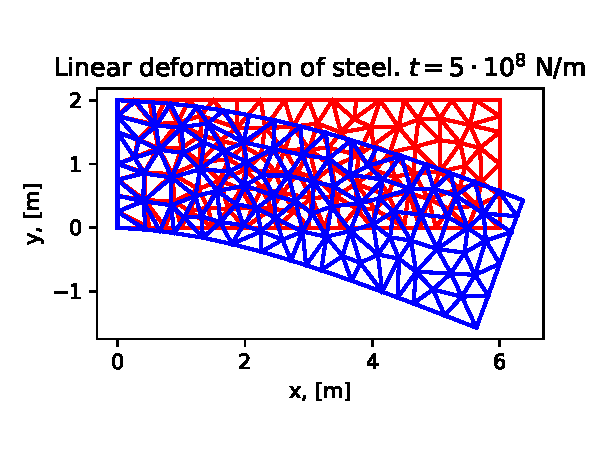
\includegraphics[width=\linewidth]{raw.pdf}
	\caption{Deformation of a steel bar. Max triangle area is 0.1 m$ ^2 $. Traction $ t = 5\D10^2 $. The material coordinates is shown in red, whilst the spatial coordinates are shown in blue.}
	\label{fig:raw}
\end{figure}
All experiments for this week will be performed on a 6 by 2 metre rectangular steel bar. Steel has a Young modulus of $ E = 69\D 10^9 \e{Pa} $ and a Poisson ratio of $ \nu = 0.3 $. The solution for a sample grid with traction $ t=5\D 10^8 $ N/m is seen in figure \ref{fig:raw}, and sure enough, the bar is deformed downwards on the right side, whilst the left stays put - just as expected.


\subsection{Examining the effects of mesh resolution on the deformation}
\begin{figure}
	\centering
	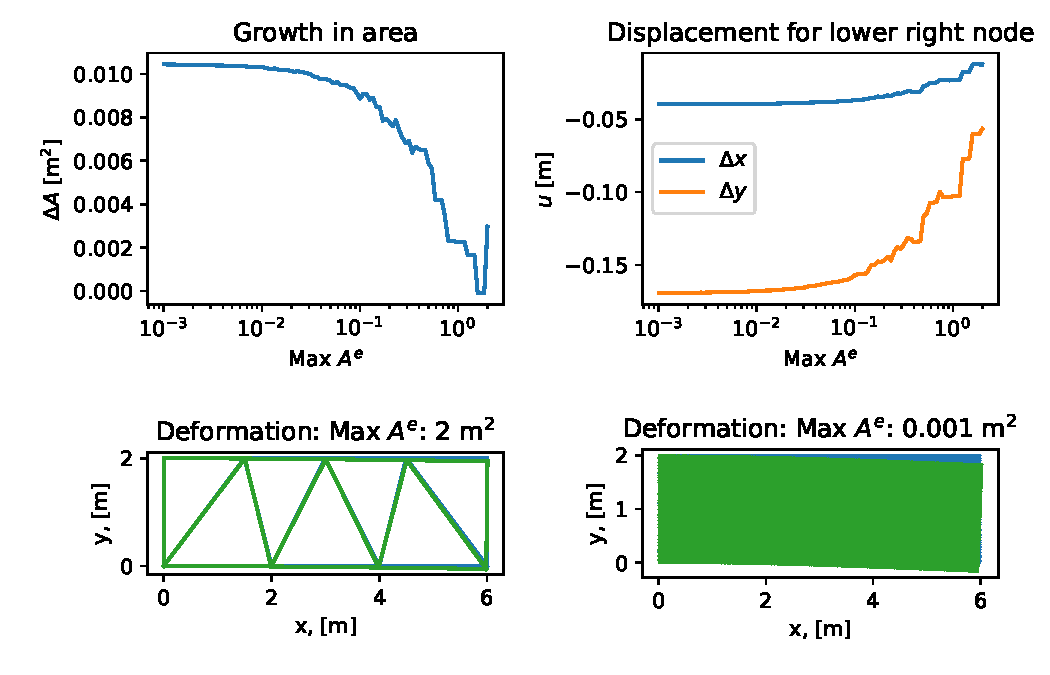
\includegraphics[width=\linewidth]{ex_resolution.pdf}
	\caption{Growth in area and displacement of the bottom right corner node, both plotted as a function of the maximum triangle area. Note the logarithmic scale on the first axis. Also shown is the deformation of the first and last mesh. Minimum angle argument set to 0, and a constant traction of $ 5\D 10^7 $ N/m was used for all simulations.}
	\label{fig:resolution}
\end{figure}
For the first experiment we test the effects of mesh resolution on the deformation of the steel bar. We set a constant traction of $ t = 5\D 10^7 $ N/m for a common point of reference between simulations. To vary the mesh resolution we pass a \texttt{.poly} file to \texttt{Triangle} with just the four corners of the bar, and lines between them, but vary the max area parameter. We perform the simulation for 50 logarithmically spaced numbers (base 2) between 2 $ \e{m}^2 $ and 0.001 $ \e{m}^2 $. For each simulation we record the difference in area between the initial and final state, along with the displacement for the lower right corner node.

We have chosen these measures for a couple of reasons: We want to evaluate whether an increase in mesh resolution will lead to a convergence upon the ``true'' value of the deformation. As such, if we want to measure the deformation, we either have to perform take some average over displacements, or just look at a single node, shared between systems. The latter is of course much easier to implement, and well behaved no matter the mesh resolution. Only four nodes are shared amongst the different meshes, namely the corners, two of which are clamped to the wall. We could of course just as well have chosen the top right node, as this would also deform, but the bottom right felt like the ``natural'' choice.

As for the area: It was an easy measure to implement, and sure enough, produces interesting results.

We expect to see convergence for both measures as the max triangle area decreases, as this increases the number of nodes and elements, and will therefore more closely model the real world (this is of course assuming the meshes generated are of sufficient quality)

The results of the experiment can be seen in figure \ref{fig:resolution}. Sure enough, the displacement of the lower right node settles towards some value as the max triangle area decreases. The same thing applies for the area of the bar, though we see a peculiar thing: one might expect the growth in area to end at a low value, not increase! It does however seem to converge upon a value, so it might just be, that this increase in area is precisely what the linear elastic deformation model predicts for a steel bar.

In the figure we have also included plots of the spatial (green) and material (blue) coordinates for the first and last mesh. The increase in displacement for the lower right node is indeed apparent from these plots as well.


\subsection{Examining the incompressibility of steel}
\begin{figure}
	\centering
	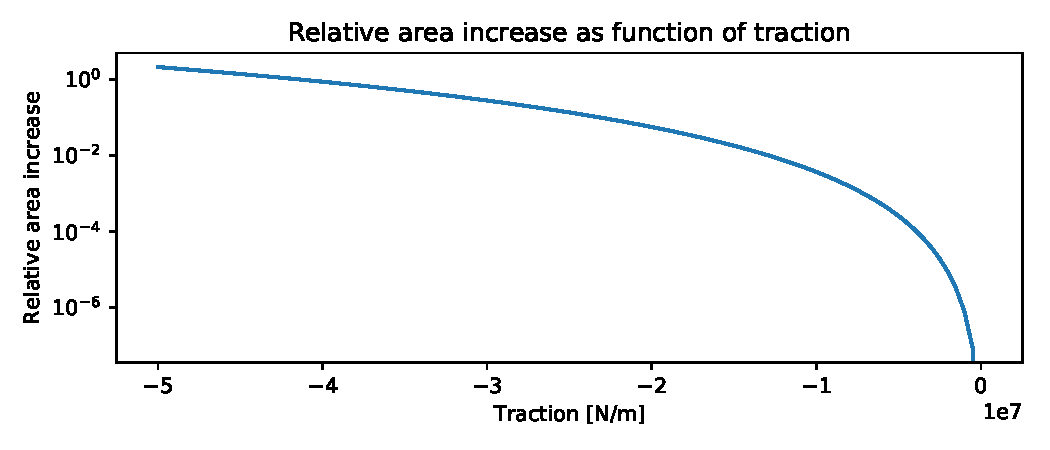
\includegraphics[width=\linewidth]{ex_loads.pdf}
	\caption{Relative area increase as a function of the traction. A mesh with max triangle area of $ 0.01 \e{m}^2 $ is used.}
	\label{fig:loads}
\end{figure}
Normally, as stated before, we would not expect steel to increase in volume/area as it experiences stresses, but the model seems to predict this. Next we perform the simulation for a range of different loads: 100 linearly spaced values between 0 and $ 5\times 10^7 $. We also choose a mesh with max triangle area 0.01 $ \e{m}^2 $. We record the area of the bar after each of the simulations, and calculate the relative area increase of the $ i $'th simulation as $ (A_i-A_0)/A_0 $. The results are seen in figure \ref{fig:loads}. We see an increase in area as indicated in the simulation before. It seems to scale like a parabola, and a look at the plot on a log-log scale reveals a strikingly linear relation between the load and relative area increase (see figure \ref{fig:logloads})
\begin{figure}
	\centering
	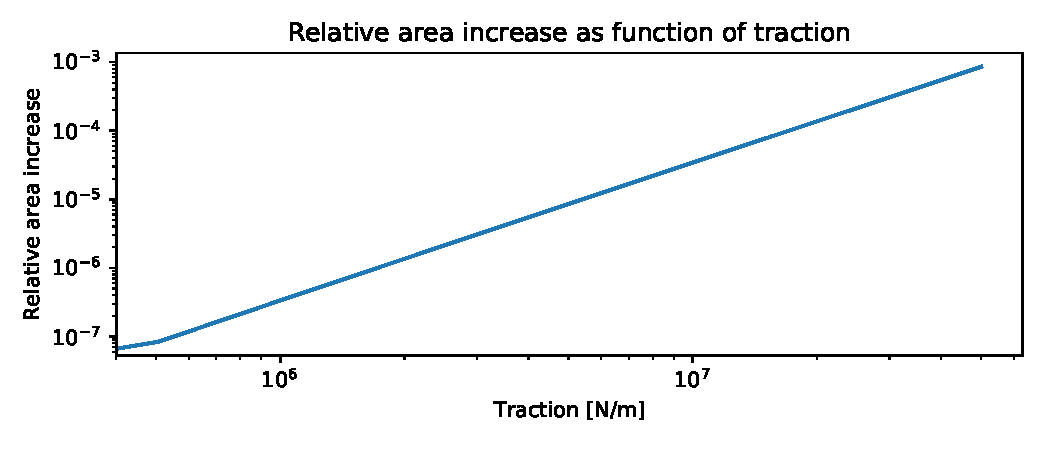
\includegraphics[width=\linewidth]{ex_logloads.pdf}
	\caption{Figure \ref{fig:loads} but for a log-log scale.}
	\label{fig:logloads}
\end{figure}
Calculating the slope is done by computing the rise over run of the values in the log-log plot:
\begin{equation}\label{eq:slope}
	\text{slope} = \frac{\log A_i - \log A_j}{\log t_i - \log t_j}
\end{equation}
for $ i > j $. We choose $ i=100, j=20 $, giving a slope of the log-log plot of 2.0012. So it is to a good approximation a parabola. Let us see, if we can make sense of it:

All non-zero values in $ f $ are the ones corresponding to nodes that experience traction, and since these values, per eq \ref{eq:boundary_elem}, scale linearly with the traction, we expect the displacement to also scale linearly since
\begin{equation*}\label{key}
	Ax=b \Rightarrow x = A\inverse b, \quad Ax' = 2b \Rightarrow x'=2A\inverse b = 2x
\end{equation*}
Now, area scales as the square of length, so a linear increase in the displacement might well induce a quadratic increase in the relative area (which of course is directly proportional to the absolute area). Of course, this is all post-hoc hypotheses based on hand-wavy arguments. To ascertain this one might more reasonably do a mathematical analysis on the increase in area as function of displacement, but I am a physicist, so I prefer doing this experimentally.

To do this experimentally, we need to vary as many different parameters as possible (one at a time, of course) and see if the effect still occurs. If it does, it is a strong hint in the direction of a quadratic relationship between the displacement and final area of the bar.

\begin{figure*}
	\centering
	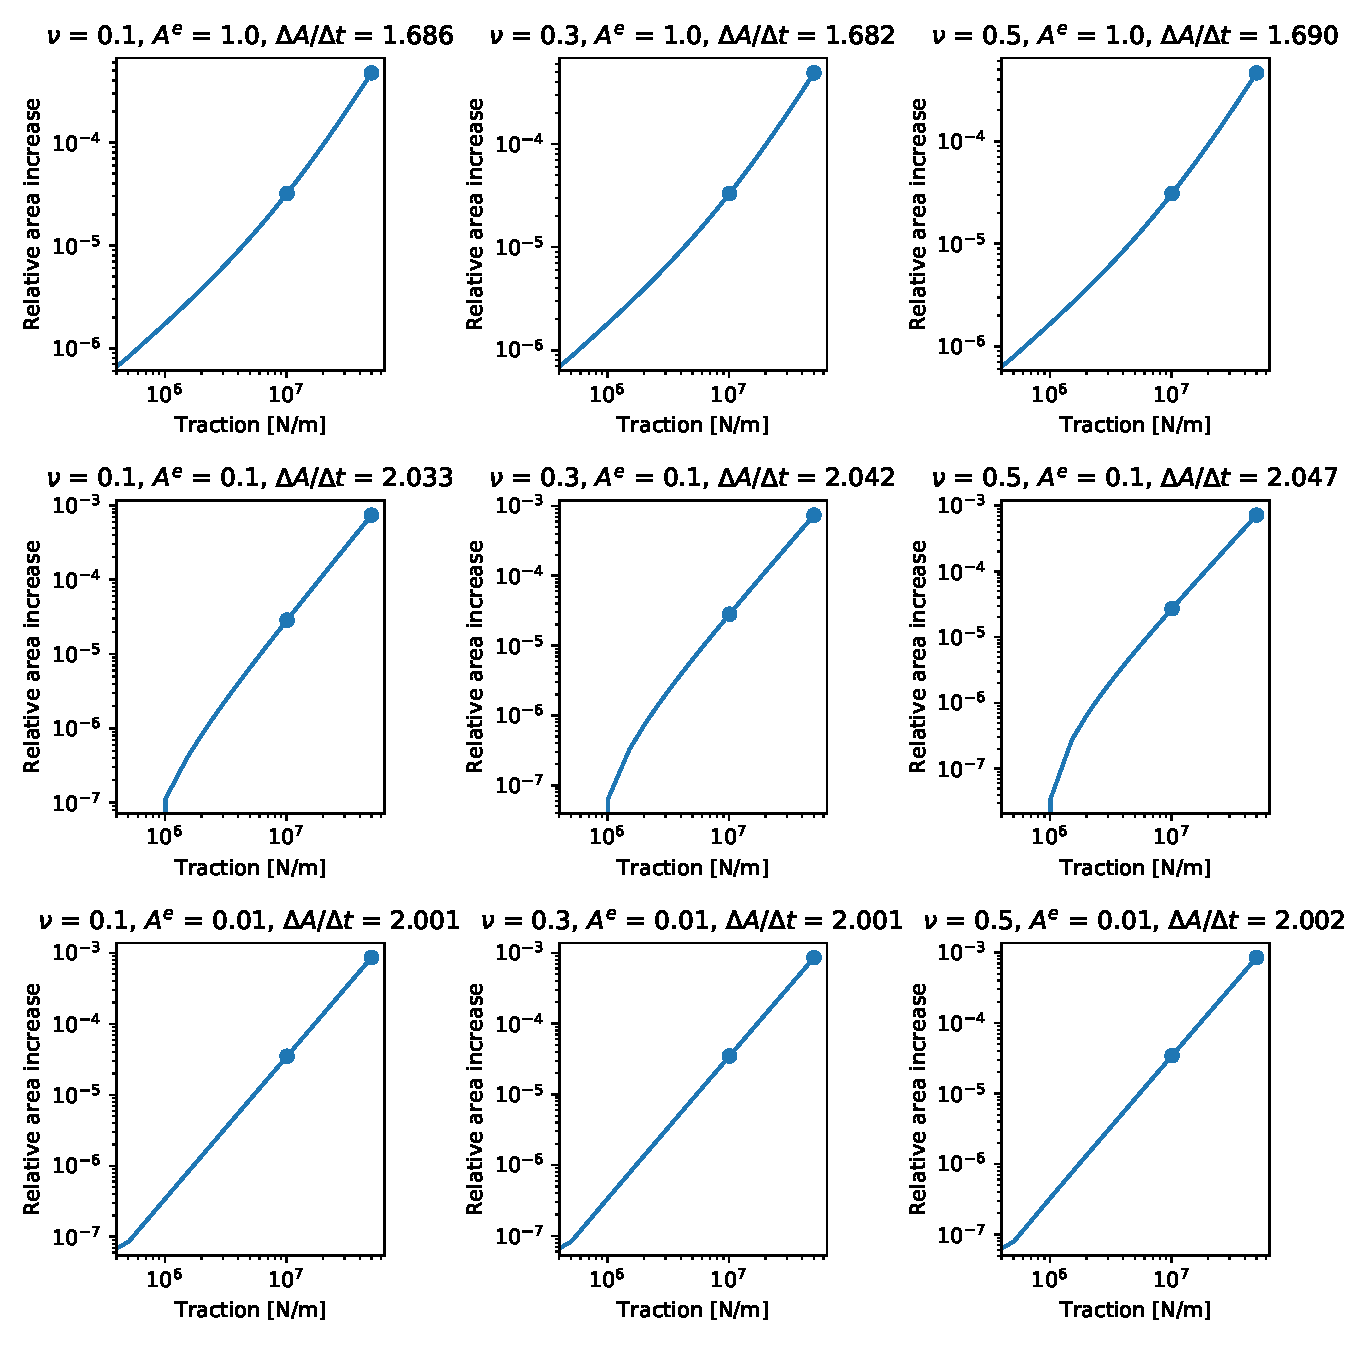
\includegraphics[width=\linewidth]{squares.pdf}
	\caption{log-log plots of traction and relative area increase, for different values of the Poisson ratio $ \nu $ and max triangle size $ A^e $. The two points shown are the ones for which the slope is calculated ($ i $=100, $ j $=20 in eq \ref{eq:slope}).}
	\label{fig:squares}
\end{figure*}
In this model we have essentially three different parameters to change: The Young modulus of the material, the Poisson ratio, and the resolution of the mesh. The Young modulus appears as a scale factor on the elasticity matrix $ D $, and as such, the displacement and Young modulus are inversely proportional:
\begin{equation*}\label{key}
	Ax=b \Rightarrow x = A\inverse b, \quad 2Ax' = b \Rightarrow x'=A\inverse b/2 = x/2
\end{equation*}
This leaves the Poisson ratio and the mesh resolution. We choose 3 different values of the Poisson ratio (0.1, 0.3, 0.5) and 3 different values of the max triangle area (1, 0.1, 0.01), and compute the relative area increase for the same range of tractions, for each set of parameter values. We then plot these on a log-log plot, which is seen in figure \ref{fig:squares}.

As seen in the figure, the relative area increase does not seem to depend on the Poisson ratio (at least not in this range of Poissons ratio), there is some deviation from the linearity of the log-log plot when varying the max triangle area. But still, for meshes of a decent resolution and up, the relationship between relative area increase and traction seems to be approximately quadratic (for large enough tractions).

Of course, this experiment only samples a small, small portion of the available parameter space, so a finer analysis of the phenomenon is warranted - a larger selection of Poisson ratios and mesh resolutions, and perhaps a proper fitting to a polynomial of some order, to get a better estimate of the relationship.

\end{document}
